\documentclass[english]{beamer}
\usepackage[T1]{fontenc}
\usepackage[latin9]{inputenc}
\setcounter{secnumdepth}{3}
\setcounter{tocdepth}{3}
\usepackage{url}
\usepackage{algorithmic}
\usepackage{algorithm}

\renewcommand{\algorithmicrequire}{\textbf{In:}}
\renewcommand{\algorithmicensure}{\textbf{Out:}}

\usepackage{amsmath}
\usepackage{amssymb}
\usepackage{caption}
\usepackage[mathscr]{eucal}
\usepackage{graphicx}
\usepackage{esint}

\makeatletter

%%%%%%%%%%%%%%%%%%%%%%%%%%%%%% LyX specific LaTeX commands.
\pdfpageheight\paperheight
\pdfpagewidth\paperwidth


%%%%%%%%%%%%%%%%%%%%%%%%%%%%%% Textclass specific LaTeX commands.
 % this default might be overridden by plain title style
 \newcommand\makebeamertitle{\frame{\maketitle}}%
 % (ERT) argument for the TOC
 \AtBeginDocument{%
   \let\origtableofcontents=\tableofcontents
   \def\tableofcontents{\@ifnextchar[{\origtableofcontents}{\gobbletableofcontents}}
   \def\gobbletableofcontents#1{\origtableofcontents}
 }

%%%%%%%%%%%%%%%%%%%%%%%%%%%%%% User specified LaTeX commands.

\usepackage{amsmath}
\usepackage{amsfonts}
\usepackage{amsthm}
\usepackage{amssymb}
%\usepackage{enumerate}
%\usepackage{etex}
%\usepackage{geometry}
\usepackage{type1cm}
 % \usepackage{calc} 
%  \usepackage{times}
%\usepackage[orientation=portrait,size=a0,scale=1.4,debug]{beamerposter}
\usepackage[orientation=landscape,size=a0, scale=1.3]{beamerposter}
   
\usepackage{natbib}
\usepackage{pifont}
\usepackage{tikz}
%\usetikzlibrary{bayesnet}

\usepackage{url}

%\usepackage{epstopdf}
%\usepackage{auto-pst-pdf}
\usepackage{subfig}
\usetikzlibrary{shapes.geometric,decorations.markings}


%\everymath{\color{mathcolor}}
%\everydisplay{\color{mathcolor}} 

% justified alignment paragraphs
\usepackage{ragged2e}   %new code
\usepackage{xcolor}
\addtobeamertemplate{block begin}{}{\justifying}  %new code

\newcommand{\diag}{\mathop{\mathrm{diag}}}
\newcommand{\trace}{\mathop{\mathrm{tr}}}
\newcommand{\median}{\mathop{\mathrm{median}}}
%\newcommand{\proj}{\mathop{\mathrm{proj}}}

\usetheme{uclposter}
%\usetheme{sharelatex}
%\useinnertheme{blockborder}

%%% increase the height of the banner: the argument is a scale factor >=1.0
\setbeamertemplate{banner}[ucl][1.1]

%%% change the colour of the main banner
%%% the background should be one of the ucl colours (except pink or white):
%%%   black,darkpurple,darkred,darkblue,darkgreen,darkbrown,richred,midred,
%%%   navyblue,midgreen,darkgrey,orange,brightblue,brightgreen,lightgrey,
%%%   lightpurple,yellow,lightblue,lightgreen,stone
\setbeamercolor{banner}{bg=lightblue, fg=black}
% \setbeamercolor{banner}{bg=yellow,fg=black}

%%% add a stripe behind the banner
% \setbeamercolor{banner stripe}{bg=brightblue,fg=black}

%%% the main structural elements
\setbeamercolor{structure}{fg=black}

%%% author/title/date and slide number in the footline
% \setbeamertemplate{footline}[author title date]

%%% puts the section/subsection in the headline
% \setbeamertemplate{headline}[section]

%%% puts a navigation bar on top of the banner
%%% for this to work correctly, the each \section command needs to be
%%% followed by a \subsection. requires one extra compile.
% \setbeamertemplate{headline}[miniframes]
%%% accepts an optional argument determining the width
% \setbeamertemplate{headline}[miniframes][0.3\paperwidth]


%%% puts the frame title in the banner
%%% won't work correctly with the above headline templates
%\useoutertheme{ucltitlebanner}
%%% similar to above, but smaller (and puts subtitle on same line as title)
% \useoutertheme[small]{ucltitlebanner}

%%% gives block elements (theorems, examples) a border
%\useinnertheme{blockborder}

%%% set a background colour
%\selectcolormodel{rgb}
%\definecolor{mylightblue}{RGB}{165, 201, 220}
\definecolor{mylightblue}{cmyk}{0.27, 0.03, 0, 0.12}
%\setbeamercolor{background canvas}{bg=mylightblue!10}
\setbeamercolor{background canvas}{bg=white}
\colorlet{mathcolor}{blue!70!black}
\setbeamercolor{normal text in math text}{fg=black}
\setbeamercolor{math text}{fg=mathcolor}
\setbeamercolor{math text displayed}{fg=mathcolor}
 \usefonttheme{professionalfonts}
\setbeamertemplate{enumerate item} {\usebeamercolor[bg]{item projected}\colorbox{bg}{\color{fg}\insertenumlabel}}

\setbeamercolor{alerted text}{fg=red}
%\setbeamercolor{background canvas}{bg=white}
%\setbeamercolor{block body alerted}{bg=normal text.bg!90!black}
\setbeamercolor{block body}{use=structure, bg=white}
%\setbeamercolor{block body example}{bg=normal text.bg!90!black}
%\setbeamercolor{block title alerted}{use={normal text,alerted text},fg=alerted text.fg!75!normal text.fg,bg=normal text.bg!75!black}
%\setbeamercolor{block title}{use=structure, bg=orange!10!white, fg=black}
%\setbeamercolor{block title example}{use={normal text,example text},fg=example text.fg!75!normal text.fg,bg=normal text.bg!75!black}
%\setbeamercolor{fine separation line}{}
%\setbeamercolor{item projected}{fg=black}
\setbeamercolor{normal text}{fg=black}

\setbeamercolor{itemize item}{fg=blue} 
\setbeamercolor{item projected}{bg=black!10!white, fg=black} 
\setbeamercolor{itemize subitem}{fg=orange} 
\setbeamertemplate{itemize item}[rectangle]  
\setbeamertemplate{itemize subitem}[circle]   %triangle
%\setbeamercolor{palette sidebar primary}{use=normal text,fg=normal text.fg}
%\setbeamercolor{palette sidebar quaternary}{use=structure,fg=structure.fg}
%\setbeamercolor{palette sidebar secondary}{use=structure,fg=structure.fg}
%\setbeamercolor{palette sidebar tertiary}{use=normal text,fg=normal text.fg}

%% \setbeamercolor{section in sidebar}{fg=brown}
%% \setbeamercolor{section in sidebar shaded}{fg= grey}
%% \setbeamercolor{separation line}{}
%% \setbeamercolor{sidebar}{bg=red}
%% \setbeamercolor{sidebar}{parent=palette primary}
%\setbeamercolor{structure}{fg=orange!90!black}

%% \setbeamercolor{subsection in sidebar}{fg=brown}
%% \setbeamercolor{subsection in sidebar shaded}{fg= grey}
%% \setbeamercolor{titlelike}{fg=brown}
%\setbeamercolor{title in head/foot}{fg=normal text.fg, bg=white}
%\setbeamercolor{author in head/foot}{fg=black}
%\setbeamercolor{math text}{fg=mathcolor}
%\setbeamercolor{math text inlined}{fg=mathcolor}

%%% set a background image
%%% some sample images are available from the ucl image store:
%%%   https://www.imagestore.ucl.ac.uk/home/start
% \setbeamertemplate{background canvas}{%
%   \includegraphics[width=\paperwidth]{imagename}}

\setbeamersize{text margin left=9cm,text margin right=-2cm}
% \newlength\blockcolsep
% \setlength\blockcolsep{2ex}
% \newlength\postercolumnsep
% \setlength\postercolumnsep{2cm}


\newlength\totalwidth
\setlength\totalwidth{\textwidth+3ex}


\newcommand{\bx}{\mathbf{x}}				% all variables
%\newcommand{\factor}{\psi}				% factor
\newcommand{\factor}{f}				% AG: made this f for consistency
\newcommand{\outV}{V}                         %AG: output variable of a factor
\newcommand{\fis}[1]{\mathrm{ne}(#1)}   	% index set for variables connected to  factor
\newcommand{\fx}[1]{ \mathbf{x}_{\mathrm{ne}(#1)} }   	% variables of a factor
\newcommand{\xin}{\mathbf{x}_{ \mathrm{in} }} 			% parents of directed factor
\newcommand{\xout}{\mathbf{x}_{ \mathrm{out} }}			% child of directed factor
\newcommand{\msg}[2]{m_{#1 \rightarrow #2}}			% message from arg1 to arg2
\newcommand{\approxMsg}[3]{M_{#1 \rightarrow #2}^{#3}}			% message from arg1 to arg2
\newcommand{\uncert}{{\mathfrak v}}          %%AG: variable used to denote uncertainty
\newcommand{\uncertaintyMsg}[3]{{\mathfrak V}_{#1 \rightarrow #2}^{#3}}			% message from arg1 to arg2
\newcommand{\diffd}{\mathrm{d}}
%\newcommand{\proj}{\mathrm{proj}}   %AG: replaced with notation using less space

%\newcommand{\proj}{\mathbb{Q}}


\newcommand{\projP}[1]{\mathrm{proj} \left [ #1 \right]}   
%\newcommand{\projP}[1]{\mathbb{Q} \left [ #1 \right]} %AG: replaced with notation using less space
\DeclareMathOperator*{\proj}{\text{proj}} % WJ defined this

\newcommand{\argmin}[1]{\mathrm{arg}\mathrm{min}_{#1}}
\newcommand{\kld}[2]{\mathrm{KL} \left [ #1 || #2 \right ]}
\newcommand{\expectationE}[2]{ \mathbb{E}_{#2}  \left[ #1 \right] }

% random features stuff
\newcommand{\feax}{\mathsf{x}}
\newcommand{\feaX}{\mathsf{X}}
\newcommand{\feay}{\mathsf{y}}
\newcommand{\feaY}{\mathsf{Y}}

\newcommand{\figref}[1]{Fig.~\ref{#1}}
\newcommand{\secref}[1]{Section~\ref{#1}}
\newcommand{\tabref}[1]{Table.~\ref{#1}}

% Gatsby Unit, University College London$^1$ \\
% \vspace*{2mm}
% University of Oxford$^2$ \\
% \texttt{ \{wittawatj,  arthur.gretton\}@gmail.com}, \, \texttt{nheess@nhuk.de} \\ 
% \texttt{ali@arkitus.com}, \, \texttt{balaji@gatsby.ucl.ac.uk},\\
% \texttt{dino.sejdinovic@gmail.com},\, \texttt{z.szabo@ucl.ac.uk}

% justifying text in itemize environments.
\renewcommand{\itemize}[1][]{%
  \beamer@ifempty{#1}{}{\def\beamer@defaultospec{#1}}%
  \ifnum \@itemdepth >2\relax\@toodeep\else
    \advance\@itemdepth\@ne
    \beamer@computepref\@itemdepth% sets \beameritemnestingprefix
    \usebeamerfont{itemize/enumerate \beameritemnestingprefix body}%
    \usebeamercolor[fg]{itemize/enumerate \beameritemnestingprefix body}%
    \usebeamertemplate{itemize/enumerate \beameritemnestingprefix body begin}%
    \list
      {\usebeamertemplate{itemize \beameritemnestingprefix item}}
      {\def\makelabel##1{%
          {%
            \hss\llap{{%
                \usebeamerfont*{itemize \beameritemnestingprefix item}%
                \usebeamercolor[fg]{itemize \beameritemnestingprefix item}##1}}%
          }%
        }%
      }
  \fi%
  \beamer@cramped%
  \justifying% NEW
  %\raggedright% ORIGINAL
  \beamer@firstlineitemizeunskip%
}

\graphicspath{{../uai2015/img/}}
%%%%%%%%%%%%%%
\title{Kernel-Based Just-In-Time Learning for Passing Expectation Propagation
    Messages \vspace{5mm} }
\author{Wittawat Jitkrittum$^1$, \, Arthur Gretton$^1$, \, Nicolas Heess, \, S. M. Ali Eslami \\
Balaji Lakshminarayanan$^1$, \, Dino Sejdinovic$^2$, and \, Zolt{\'a}n Szab{\'o}$^1$  
\vspace*{2mm} 
}
\institute{%
Gatsby Computational Neuroscience Unit, University College London$^1$ 
\hspace{2cm}
University of Oxford$^2$
%\newline Google DeepMind$^2$
}


\setbeamerfont{footline}{size=\fontsize{20}{24}\selectfont}
\setbeamertemplate{footline}
{
  \leavevmode%
  \hbox{%
  \begin{beamercolorbox}[wd=.5\paperwidth,ht=2.25ex,dp=1ex]{author in head/foot}%
    \usebeamerfont{author in head/foot} \hspace{0.5cm} We gratefully acknowledge the support of the Gatsby Charitable Foundation.
  \end{beamercolorbox}%
  \begin{beamercolorbox}[wd=.5\paperwidth,ht=2.25ex,dp=1ex]{title in head/foot}%
    \usebeamerfont{title in head/foot} Email: \texttt{wittawat@gatsby.ucl.ac.uk} \hspace*{2cm} Homepage: \texttt{wittawat.com}
  \end{beamercolorbox}}%
  \vskip0pt%
}

\makeatother

\usepackage{babel}

\newenvironment{wideitemize}{\itemize\addtolength{\itemsep}{100pt}}{\enditemize}
%%%%%%%%%%%%%%%%%%%%%%%%%%%%%%%%%%%%%%
\begin{document}

\newcommand{\Simley}[2]{%
\begin{tikzpicture}[scale=0.5]
    \newcommand*{\SmileyRadius}{1.1}%
    \draw [fill=#2] (0,0) circle (\SmileyRadius)% outside circle
        %node [yshift=-0.22*\SmileyRadius cm] {\tiny #1}% uncomment this to see the smile factor
        ;  
    \pgfmathsetmacro{\eyeX}{0.5*\SmileyRadius*cos(30)}
    \pgfmathsetmacro{\eyeY}{0.5*\SmileyRadius*sin(30)}
    \draw [fill=cyan,draw=none] (\eyeX,\eyeY) circle (0.15cm);
    \draw [fill=cyan,draw=none] (-\eyeX,\eyeY) circle (0.15cm);
    \pgfmathsetmacro{\xScale}{2*\eyeX/180}
    \pgfmathsetmacro{\yScale}{1.0*\eyeY}
    \draw[color=red, domain=-\eyeX:\eyeX]   
        plot ({\x},{
            -0.1+#1*0.15 % shift the smiley as smile decreases
            -#1*1.75*\yScale*(sin((\x+\eyeX)/\xScale))-\eyeY});
\end{tikzpicture}%
}% 

% \newcommand{\Smile}{\Simley{0.6}{green!20}}
% \newcommand{\Frown}{\Simley{-0.53}{red!15}}
\newcommand{\cmark}{\ding{51}}%
\newcommand{\xmark}{\ding{55}}%
\newcommand{\Smile}{ {\large \textcolor{green}{\cmark}} }
\newcommand{\Frown}{ {\large \textcolor{red}{\xmark}} }

\newcommand{\Vskip}{\vspace{5mm}}
\begin{frame}


\begin{columns}[t]

%==================================
\column{0.31\textwidth}
%==================================

%%--------------------------
%\begin{block}{Introduction }
%%--------------------------

%\justifying{}Two approaches to automated probabilistic inference
%{[}3{]}:
%\begin{enumerate}
%\item \justifying{}\textbf{Uninformed}: 


%\Vskip{}\Smile{} Free to use any factors to express a model.


%\Vskip{}\Frown{} Typically rely on MCMC-based sampling techniques.
%Slow.

%\item \textbf{Informed}: 


%\Vskip{}\Smile{} Models built from handcrafted factors known to the
%inference engine e.g., Infer.NET {[}4{]}. Efficient inference. 


%\Vskip{}\Frown{} Use of unsupported factors requires manual derivation
%of message updates. 

%\end{enumerate}
%\end{block}

%--------------------------
\begin{block}{Contribution }
%--------------------------

Propose to incrementally learn during inference a kernel-based EP message operator 
(distribution-to-distribution regression)
%
\begin{equation*}
    \left[ m_{V'\rightarrow f}  \right]_{V' \in \mathrm{ne}(f)} \mapsto q_{f \rightarrow V}
\end{equation*}
%
for any factor $f$ that can be sampled. 
%Outgoing message 
%$m_{f \rightarrow V} := q_{f \rightarrow V} / m_{V \rightarrow f}$ can be computed easily.

%Bridge the gap between the two approaches. 

%\Vskip{}\Smile{} No constraint on the set of usable factors.

%\Vskip{}\Smile{} Message updates automatically learned online (just in time).

%\Vskip{}\Smile{} Novel two-layer random feature representation of input
%messages for fast message updates.

%\Vskip{}\Smile{} The operator can ask the oracle and incorporate new input
%messages when it is uncertain.

\vspace*{3mm}
\textbf{Merits}:
\begin{itemize}
%\item No constraint on the set of usable factors.

\item  Efficient message updates: 
    \begin{itemize}
        \item Learned online (just in time).
        \item Two-layer random kitchen sinks 
    \end{itemize}

\item Operator: uncertainty aware

%    The operator can ask the oracle and incorporate new input
%messages when it is uncertain.
\end{itemize}

\end{block}

%--------------------------
\begin{block}{Expectation Propagation (EP)}
%--------------------------
Under an approximation that each factor fully factorizes, an outgoing EP message $m_{f\rightarrow V}$ takes the form
\vspace{15mm}
%% \begin{align*}
%% \frac{\proj\left[\int d\mathcal{V}\backslash\{v\}\, f(\mathcal{V})\prod_{V'\in\mathcal{V}}m_{V'\rightarrow f}(v')\right]}{m_{V\rightarrow f}(v)}:=\frac{q_{f\rightarrow V}(v)}{m_{V\rightarrow f}(v)}
%% \end{align*}
 
\tikzstyle{every picture}+=[remember picture]
\tikzstyle{na} = [baseline=-.5ex]

%\tikz[na] \node[fill=blue!10,draw,circle] (n1) {}; 
\begin{tikzpicture}[scale=1]
\draw[help lines, white] (0, -1) grid (25, 2); 
%\draw[very thick, <->] (1,0) to (0,0) to (0,1); 
\node (v_def) [right, fill=orange!20, inner sep=10pt, align=center, text
width=9cm] at (3, 0) {set of $c$ variables connected to $f$};
\node (proj_msg_def) [right, fill=green!20, ellipse, inner sep=1pt,
align=center, text width=5cm] at (18, 0) {projected message};
\end{tikzpicture}

\begin{align*}
  m_{f\rightarrow V}(v) = 
  \frac{
	  \tikz[baseline]{
	  \node[fill=blue!7,anchor=base] (proj){ $\proj$ };
  }
  \left[\int d\mathcal{V}\backslash\{v\}\, f(
	  \tikz[baseline]{
		  \node[fill=orange!20,anchor=base, inner sep=3pt] (v_set){$\mathcal{V}$};
	  }
  )\prod_{V'\in\mathcal{V}} 
	  \tikz[baseline]{
		  \node[fill=red!20!white,anchor=base] (inc) 
		  {$m_{V'\rightarrow f}(v')$}; % end numerator
	  }
  \right]}{m_{V\rightarrow f}(v)} := 
  \frac{	
  \tikz[baseline]{
	  \node[fill=green!20,anchor=base] (projected)
	  { $q_{f\rightarrow V}(v)$ };
  }
  }{m_{V\rightarrow f}(v)}  
\end{align*}

\begin{tikzpicture}[scale=1]
\draw[help lines, white] (0, -1) grid (25, 2);
%\draw[very thick, <->] (1,0) to (0,0) to (0,1); 
\node (projdef) [right, fill=blue!7, rectangle, inner sep=12pt, align=center,
text width=20cm]  at (0.5, 0) {$\proj[r_{f \rightarrow
V}]:=\arg\min_{q\in\text{ExpFam}}\text{KL}\left[r_{f \rightarrow V}\,\|\,
q\right]$ (projection onto exponential family)}; 
%
\node (incdef) [right, fill=red!20, ellipse, inner sep=1pt, align=center, text
width=5cm]  at (23, 0) {incoming message from $V'$}; 
\end{tikzpicture}


% Now it's time to draw some edges between the global nodes. Note that we
% have to apply the 'overlay' style.
\begin{tikzpicture}[overlay]
	\draw[->, line width=3pt] (v_def) edge [bend left] (v_set.north);
    %\draw[->, line width=3pt] (projdef.north) to [out=120, in=-90] (proj.south);
    \draw[->, line width=3pt] (projdef) to [bend left] (proj.south);
    \path[->, line width=3pt] (incdef) edge [bend left] (inc);
    %\path[->, line width=4pt] (proj_msg_def) edge [out=80, in=220] (projected.south west);
    \path[->, line width=3pt] (proj_msg_def) edge [bend left] (projected.north);
\end{tikzpicture}

%% \begin{tikzpicture}[scale=1.5]
%% \node at (0,0) {
%% {\Large $  m_{f\rightarrow V}(v) = \frac{
%% \proj
%% \left[\int d\mathcal{V}\backslash\{v\}\, f(\mathcal{V})\prod_{V'\in\mathcal{V}}m_{V'\rightarrow f}(v')\right]}
%% {m_{V\rightarrow f}(v)} 
%% :=\frac{q_{f\rightarrow V}(v)}{m_{V\rightarrow f}(v)} $ }
%% };
%% \end{tikzpicture}

\vspace{-20mm}
\begin{figure}[ht]
\centering
  \subfloat[ Message passing on a factor graph.]{
  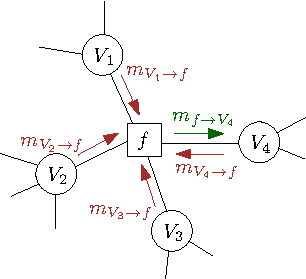
\includegraphics[width=0.45\columnwidth]{img/factor_graph-crop.pdf}
  }
  %
  \subfloat[ Projection of $r_{f\rightarrow V}$ to a Gaussian]{
  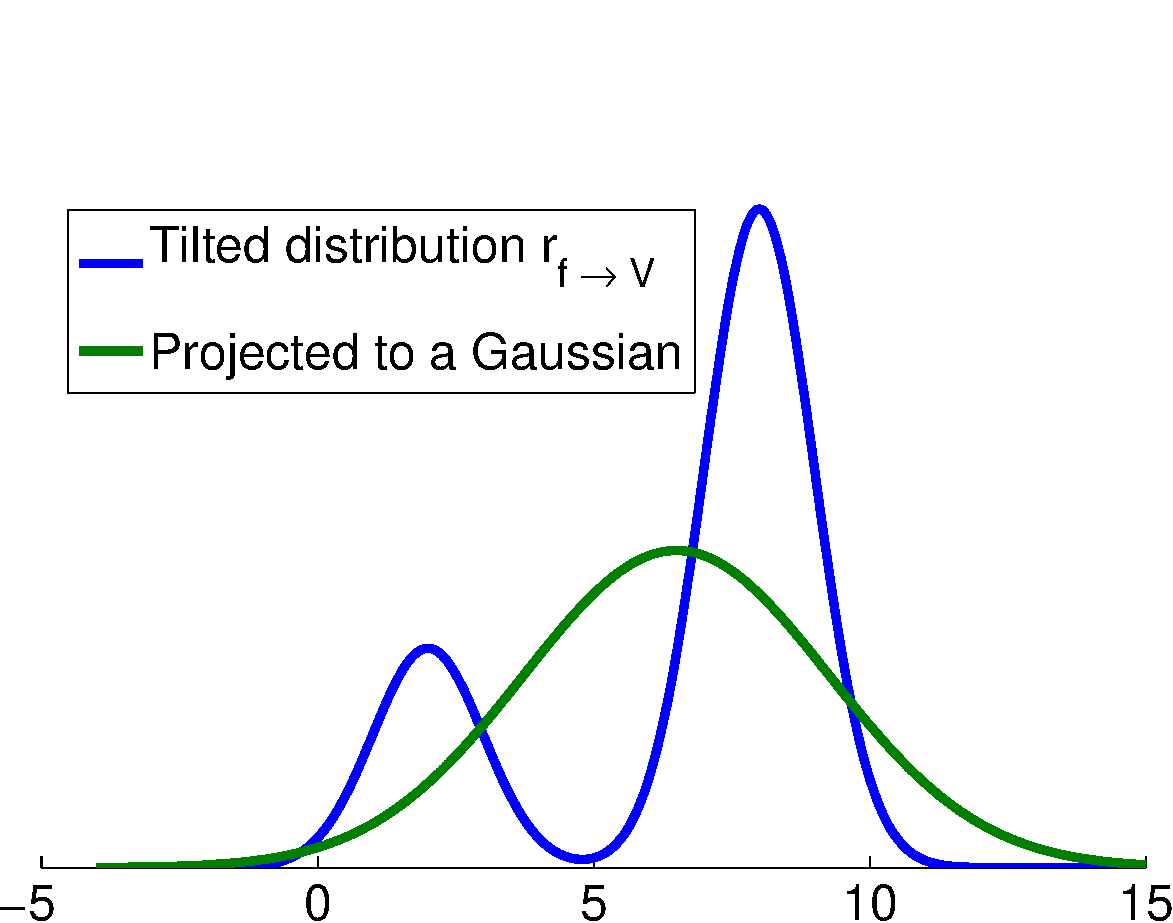
\includegraphics[width=0.45 \columnwidth]{img/proj_demo-crop.pdf}
  }
  %
\end{figure}
%
\vspace{1cm}
\textbf{Projected message:} 

\begin{itemize}
    \item $q_{f\rightarrow V}(v)=\proj\left[r_{f\rightarrow V}(v)\right] \in
        \text{ExpFam}$ with sufficient statistic $u(v)$

    \item Moment matching: $\mathbb{E}_{q_{f\rightarrow
        V}}\left[u(v)\right]=\mathbb{E}_{r_{f\rightarrow V}}\left[u(v)\right] $
\end{itemize}

%Let $q_{f\rightarrow V}(v)\in\text{ExpFam}$
%with sufficient statistic $u(v)$. 


%\begin{equation*}
%\mathbb{E}_{q_{f\rightarrow V}}\left[T(v)\right]=\mathbb{E}_{r_{f\rightarrow V}}\left[T(v)\right] \text{(moment matching).}
%\end{equation*}
%
\end{block}

%--------------------------
\begin{block}{Kernel on Incoming Messages}
%--------------------------

\begin{itemize}
    \item Joint distribution from $c$ incoming messages: 
        $\mathsf{r}:=\times_{l=1}^c r_{l}$, \hspace{5mm}
        $\mathsf{s}:=\times_{l=1}^c s_{l}$     
    
    \item Mean embedding of $\mathsf{r}$:
        $\mu_{\mathsf{r}}:=\mathbb{E}_{a \sim \mathsf{r}}k(\cdot,a)$ 

    \item Gaussian Kernel: 
        \begin{align*}
            \kappa(\mathsf{r}, \mathsf{s}) &= 
            \exp\left(-\frac{\|\mu_{\mathsf{r}}-\mu_{\mathsf{s}}\|_{\mathcal{H}}^{2}}{2\gamma^{2}}\right). 
%&= \exp\left(-\frac{1}{2\gamma^{2}}\left\langle
%  \mu_{\mathsf{r}},\mu_{\mathsf{r}}\right\rangle
%  +\frac{1}{\gamma^{2}}\left\langle
%  \mu_{\mathsf{r}},\mu_{\mathsf{s}}\right\rangle
%  -\frac{1}{2\gamma^{2}}\left\langle
%  \mu_{\mathsf{s}},\mu_{\mathsf{s}}\right\rangle \right).
        \end{align*}

\end{itemize}
%
%\begin{align*}
% %\kappa_{\text{gauss}}(p,q) \\
%    \kappa(\mathsf{r}, \mathsf{s}) = 
%  \exp\left(-\frac{1}{2\gamma^{2}}\left\langle
%  \mu_{\mathsf{r}},\mu_{\mathsf{r}}\right\rangle
%  +\frac{1}{\gamma^{2}}\left\langle
%  \mu_{\mathsf{r}},\mu_{\mathsf{s}}\right\rangle
%  -\frac{1}{2\gamma^{2}}\left\langle
%  \mu_{\mathsf{s}},\mu_{\mathsf{s}}\right\rangle \right).
%  %
%\end{align*}
%
\end{block}
%==================================
\column{0.3\textwidth}
%==================================

Two-Staged Random Feature Approximations
\begin{equation*}
    \kappa(\mathsf{r},
    \mathsf{s})\approx\exp\left(-\frac{
        \|\hat{\phi}(\mathsf{r})-\hat{\phi}(\mathsf{s})\|_{D_\mathrm{in}}^{2}}{2\gamma^{2}}\right)
        \approx
        \hat{\psi}(\mathsf{r})^\top \hat{\psi}(\mathsf{s}).
    \end{equation*}

%--------------------------
\begin{block}{Message Operator }
%--------------------------
Bayesian linear regression:

\begin{itemize}
    \item \textbf{Input:} $\mathsf{X}=\left(\mathsf{x}_{1}|\cdots|\mathsf{x}_{N}\right)$: 
        $N$ training incoming messages represented as random feature vectors.
    \item \textbf{Output:} $\mathsf{Y}=\left(\mathbb{E}_{r_{\factor\rightarrow
        \outV}^{1}}u(x_{\outV})|\cdots|\mathbb{E}_{r_{f\rightarrow
        \outV}^{N}}u(x_{\outV})\right)\in\mathbb{R}^{D_{y}\times N}$: 
        sufficient statistics of outgoing messages.
    \item Inexpensive online update
    \item Uncertainty estimate: predictive variance
\end{itemize}

%
%\small
%\begin{align*}
%    w & \sim\mathcal{N}\left(w;0,I_{D_\mathrm{out}}\sigma_{0}^{2}\right) & \text{prior}  \\
%    \mathsf{Y} \mid \mathsf{X},w & \sim\mathcal{N}\left(\mathsf{Y};w^{\top}
%    \mathsf{X},\sigma_{y}^{2}I_{N}\right) & \text{likelihood}\\
%%
%    p(w | \mathsf{Y}) & =\mathcal{N}(w;\mu_{w},\Sigma_{w}) & \text{posterior of } w \\
%    %
%    \Sigma_{w} & = \left( \mathsf{X}
%    \mathsf{X}^{\top}\sigma_{y}^{-2}+\sigma_{0}^{-2}I \right)^{-1} 
%    & \text{posterior covariance}\\
%    %
%    \mu_{w} & =\Sigma_{w} \mathsf{X} \mathsf{Y}^{\top}\sigma_{y}^{-2}. 
%    & \text{posterior mean }\\
%% predictive
%    p(\mathsf{y}^{*}| \mathsf{x}^{*}, \mathsf{Y}) 
%    & =\mathcal{N}\left(\mathsf{y}^{*}; \mathsf{x}^{*\top}\mu_{w},
%    \mathsf{x}^{*\top}\Sigma_{w} \mathsf{x}^{*}+\sigma_{y}^{2}\right)
%    & \text{predictive dist.}
%\end{align*}

%\textbf{Uncertainty Awareness}
%If $\mathsf{x}^{*\top}\Sigma_{w} \mathsf{x}^{*}+\sigma_{y}^{2} \leq $
%uncertainty threshold, $m_{f \rightarrow V}$ is efficiently predicted.
%Otherwise, update the operator with $(x^*, y^*)$ where $y^* =\mathbb{E}_{r_{f
%\rightarrow V}}[u(v)] $ is obtained by importance sampling.

%Posterior covariance at time $N+1$:
%%
%\begin{equation*}
%\Sigma_{w}^{(N+1)} 
% =
%\Sigma_{w}^{(N)}-\frac{\Sigma_{w}^{(N)} \mathsf{x}_{N+1}
%\mathsf{x}_{N+1}^{\top} \Sigma_{w}^{(N)}\sigma_{y}^{-2}}{1+
%    \mathsf{x}_{N+1}^{\top}\Sigma_{w}^{(N)} \mathsf{x}_{N+1}\sigma_{y}^{-2}}.
%\end{equation*}
%
%which is an inexpensive update of covariance at time $N$.

\end{block}


%--------------------------
\begin{block}{Two-Staged Random Features }
%--------------------------
% \begin{algorithm}[t]
% \caption{Construction of two-stage random features for $\kappa$}
% \label{algo:random_features_kgg}
\begin{algorithmic}[1]
\REQUIRE 
%Joint $\mathsf{r}$ of incoming messages, 
$\mathscr{F}(k)$: Fourier transform of $k$, $D_\mathrm{in}$: \#inner features, 
$D_\mathrm{out}$: \#outer features 
%, outer Gaussian width $\gamma^2$.
\ENSURE Random features $\hat{\psi}(\mathsf{r}) \in \mathbb{R}^{D_\mathrm{out}}$

%\STATE Compute the Fourier transform $\hat{k}$ of the kernel $k$.
\STATE Sample  $\{ \omega_i \}_{i=1}^{D_\mathrm{in}} \overset{i.i.d}{\sim} \mathscr{F}(k)$, 
\hspace{10mm} $\{b_i\}_{i=1}^{D_\mathrm{in}} \overset{i.i.d}{\sim} U[0, 2\pi] $.

%\STATE Sample $\{b_i\}_{i=1}^{D_\mathrm{in}} \overset{i.i.d}{\sim} U[0, 2\pi] $.
\STATE $\hat{\phi}(\mathsf{r}) = \sqrt{\frac{2}{D_\mathrm{in}}} \left(
\mathbb{E}_{\mathsf{x \sim \mathsf{r}}} 
\cos(\omega_{i}^{\top}x+b_{i} ) \right)_{i=1}^{D_\mathrm{in}} \in \mathbb{R}^{D_\mathrm{in}}$ \\
%\STATE  $\hat{\phi}(p)=\mathbb{E}_{p(x)}\sqrt{\frac{2}{D_\mathrm{in}}}\left(\cos\left(\omega_{1}^{\top}x+b_{1}\right),\ldots,\cos\left(\omega_{D_\mathrm{in}}^{\top}x+b_{D_\mathrm{in}}\right)\right)^{\top}$.
%If $\mathsf{r}(x)=\mathcal{N}(x;m, \Sigma )$,  \\
%$\hat{\phi}( \mathsf{r}) =  \sqrt{\frac{2}{D_\mathrm{in}}} \left( \cos(\omega_{i}^{\top}m +b_{i}) \exp 
%\left(-\frac{1}{2}\omega_{i}^{\top}\Sigma \omega_{i} \right) \right)_{i=1}^{D_\mathrm{in}}$.
% \small
% \begin{equation*}
% \hat{\phi}( \mathsf{r}) = \sqrt{\frac{2}{D_\mathrm{in}}} \left( \cos(\omega_{i}^{\top}m +b_{i}) \exp 
% \left(-\frac{1}{2}\omega_{i}^{\top}\Sigma \omega_{i} \right) \right)_{i=1}^{D_\mathrm{in}}.
% \end{equation*}
%
%Even if $p$ is not a normal distribution, we may still use it as an approximation.
%
\STATE Sample $\{ \nu_i \}_{i=1}^{D_\mathrm{out}} \overset{i.i.d}{\sim}
\mathscr{F}({k}_{\text{gauss}}(\gamma^{2}))$, \hspace{10mm} 
$\{c_i\}_{i=1}^{D_\mathrm{out}} \overset{i.i.d}{\sim} U[0, 2\pi] $.
%i.e., Fourier transform of a Gaussian kernel with width $\gamma^2$.
\STATE $\hat{\psi}(\mathsf{r}) = \sqrt{\frac{2}{D_\mathrm{out}}} \left(  
\cos(\nu_{i}^{\top} \hat{\phi}(\mathsf{r}) + c_{i} ) \right)_{i=1}^{D_\mathrm{out}} \in 
\mathbb{R}^{D_\mathrm{out}}$
\end{algorithmic}
% \end{algorithm}

\end{block}


%--------------------------
\begin{block}{ Experiment 1: Uncertainty Estimates}
%--------------------------

\begin{center}
%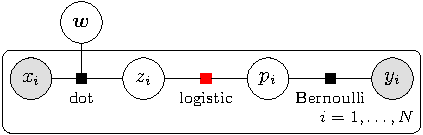
\includegraphics[width=20cm]{binary_logistic_regression-crop}
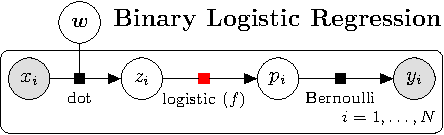
\includegraphics[width=21cm]{img/binlog_graph_title-crop}
\end{center}

\begin{itemize}

\item Approximate the logistic factor $f$: 
    %$f(z|x)=\delta\left(z-\frac{1}{1+\exp(-x)}\right)$.  Two incoming messages:
    %$\msg{z_i}{\factor} = \mathcal{N}(z_i; \mu, \sigma^2)$ and 
    %$\msg{p_i}{\factor} = \text{Beta}(p_i; \alpha, \beta) $. 
    \begin{align*}
    f(z|x) &= \delta\left(z-\frac{1}{1+\exp(-x)}\right)  \\
    \msg{z_i}{\factor} &= \mathcal{N}(z_i; \mu, \sigma^2) \\
    \msg{p_i}{\factor} &= \text{Beta}(p_i; \alpha, \beta). 
    \end{align*}
    \vspace{-10mm}

\item Training set = messages collected from 20 EP runs on toy data.

\begin{figure}[ht]
\centering
  \subfloat[Parameters of $\msg{z_i}{\factor}$ \label{fig:logistic_uncertainty_test}]{
  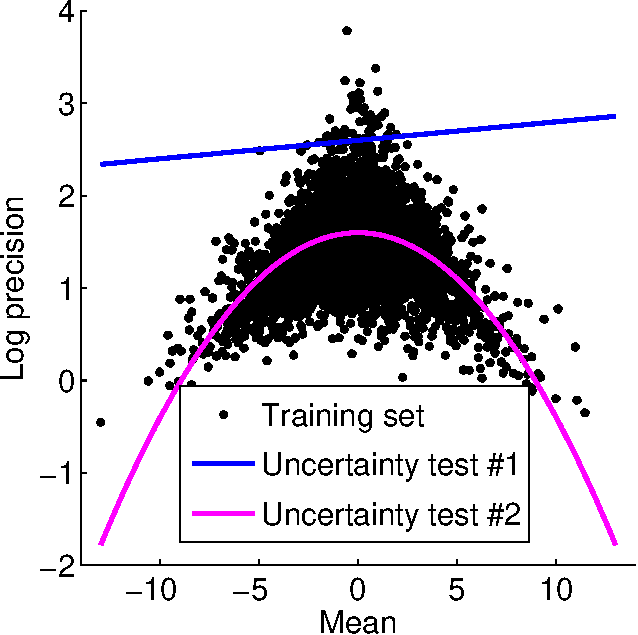
\includegraphics[width=14cm]{uncertainty/logistic_uncertainty_test-crop}
  }
  \hspace{2cm}
  %
  \subfloat[Uncertainty estimates \label{fig:logistic_uncertainty_all}]{
  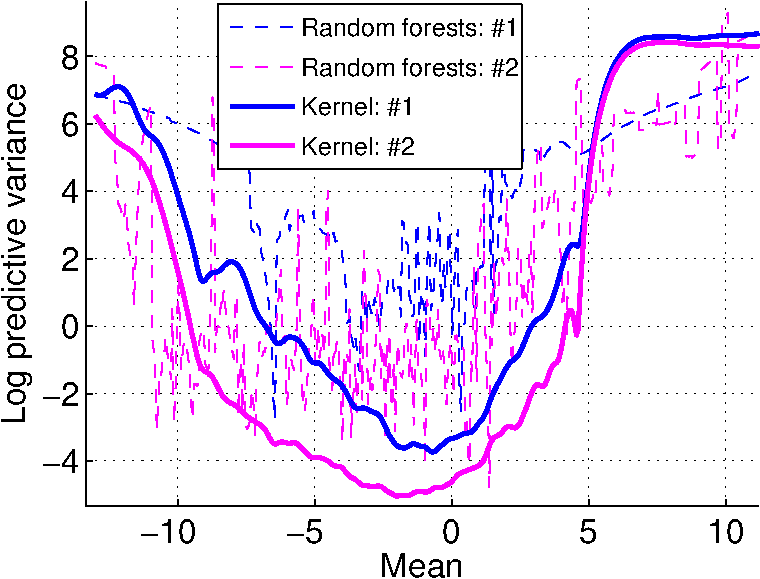
\includegraphics[width=14cm]{uncertainty/logistic_uncertainty_all-crop}
  \hspace{1.5cm}
  }
  %
  %\caption{   
  %Eslami et. al.'s random forests (KL-based agreement of predictions of different trees) 
  %on the two uncertainty test sets shown. For testing, we fix the other incoming message 
  %%$\msg{p_i}{\factor}$ to $\text{Beta}(p_i; 1, 2)$.
  %}

  %\label{fig:logistic_uncertainty}
\end{figure}

\item \#Random features: $D_{in} = 300$ and $D_{out} = 500$.
\end{itemize}



% \begin{figure}[ht]
%   \centering
% 
%   \subfloat[KL errors \label{fig:kl_div_hist}]{
%   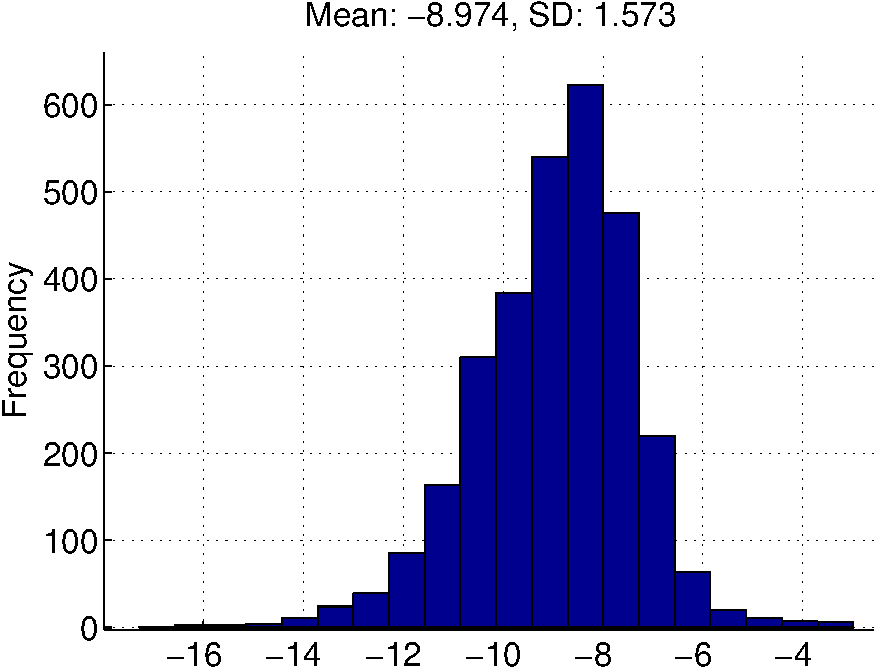
\includegraphics[width=0.3\columnwidth]{kl_ntr5000_iter5_sf1_st20_fm_joint-crop}
%   }
%   %
%   \subfloat[Examples of predictions\label{fig:kl_div_4plots}]{
%   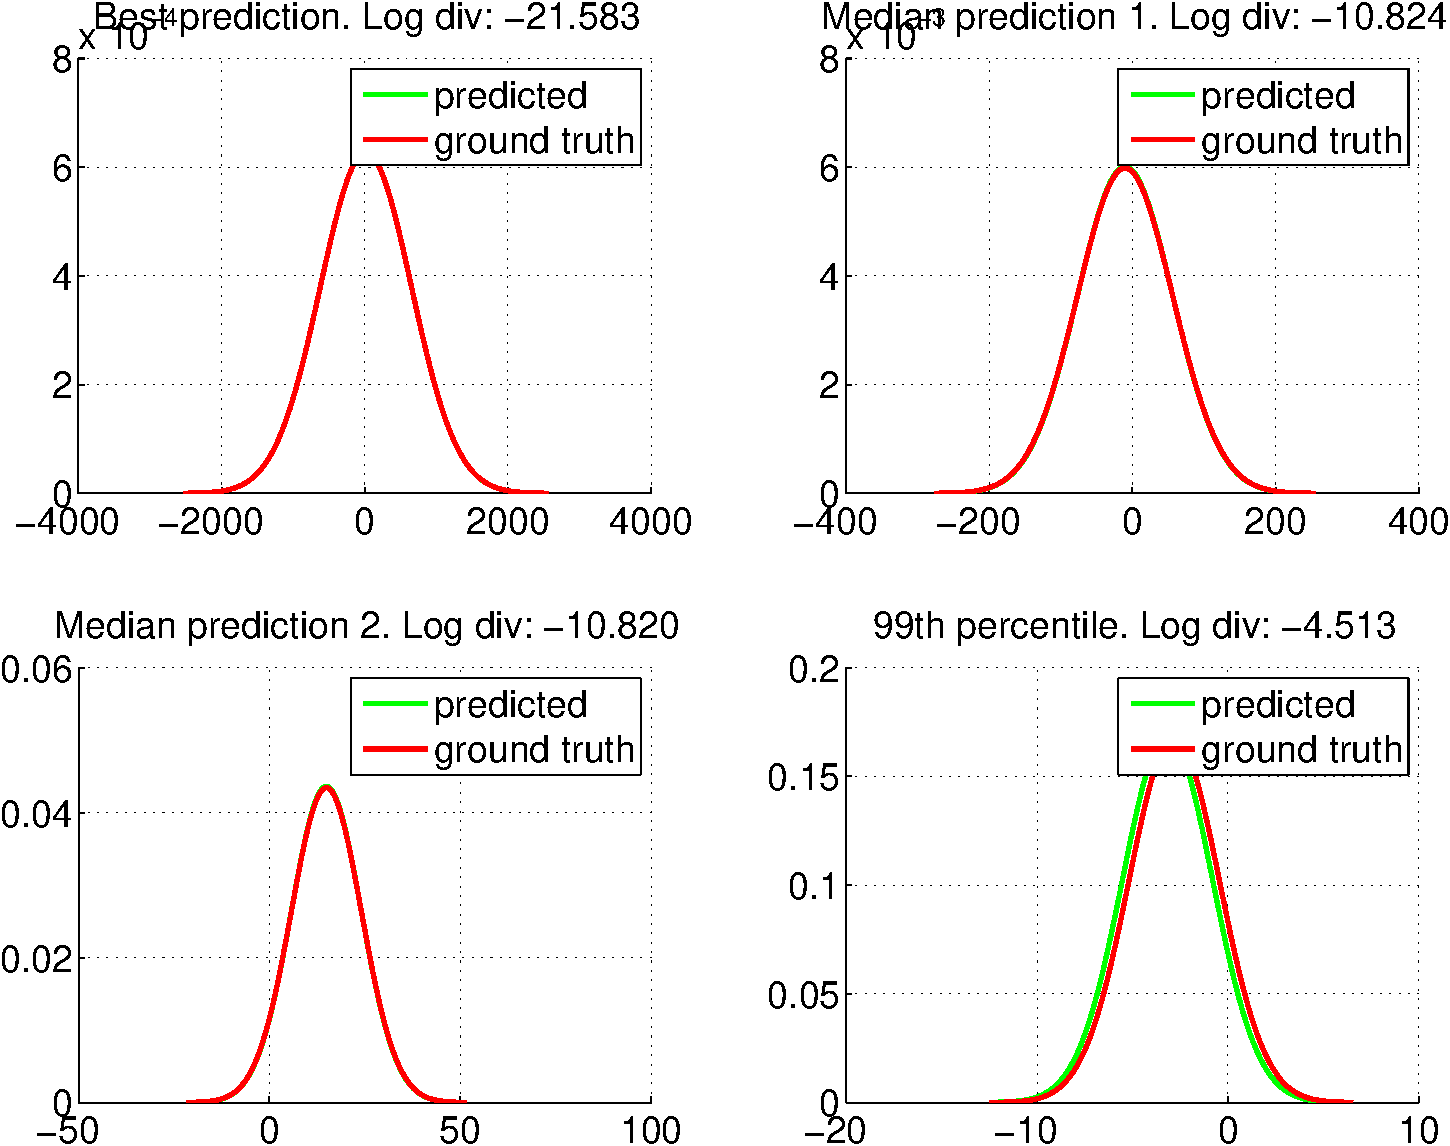
\includegraphics[width=0.3\columnwidth]{4plots_ntr5000_iter5_sf1_st20_fm_joint-crop}
%   }
%   \caption{Prediction errors for predicting the projected beliefs to $z_i$, and examples of predicted messages at different error levels. 
%   }
%   % reference: exp7/RFGJointKGGLearner_binlogis_bw_proj_n400_iter5_sf1_st20_ntr5000.mat
%   \label{fig:kl_div}
% \end{figure}



\end{block}




%==================================
\column{0.38\textwidth} 
%==================================

%--------------------------
\begin{block}{ Experiment 2: Classification Errors}
%--------------------------

% logistic temporal uncertainty
% \begin{figure}[t]
% \centering
% 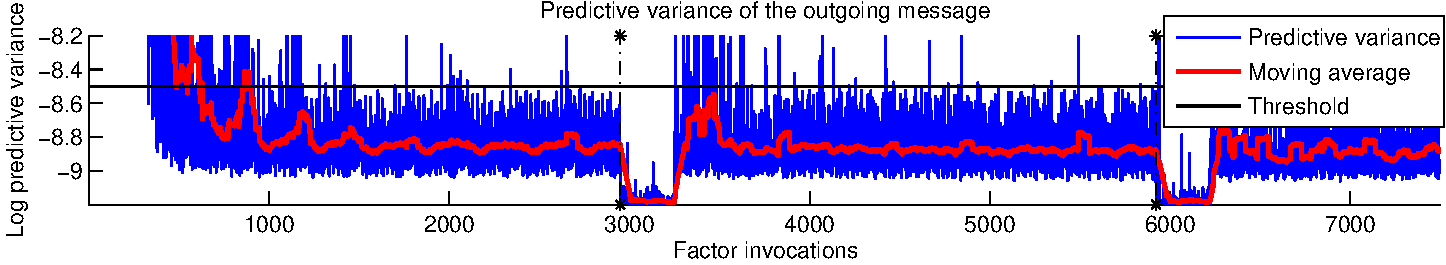
\includegraphics[width=0.95\textwidth]{online/logistic_temporal_uncertainty-crop}
% \caption{Uncertainty estimate of KJIT in its prediction of outgoing messages at each factor invocation,
% for the binary logistic regression problem. The black dashed lines indicate the start 
% of a new inference problem.
% \label{fig:logistic_temporal_uncertainty}
% }
% \end{figure}

    Fix true $\boldsymbol{w}$. Sequentially present 30 problems. Generate
    $\{(x_i, y_i\}_{i=1}^{300}$ for each.  
        %
\begin{figure}[ht]
    \vspace{5mm}
  \centering
  \subfloat[Test error \label{fig:logistic_01_loss}]{
  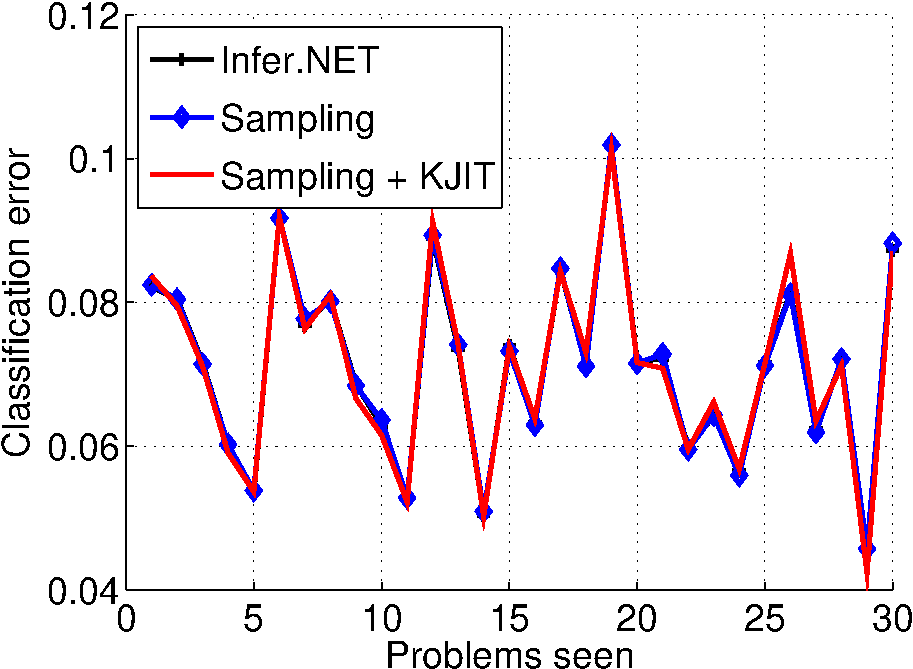
\includegraphics[width=14cm]{online/logistic_01_loss-crop}
  }
  \hspace{5mm}
  \subfloat[Inference time\label{fig:logistic_inference_time}]{
  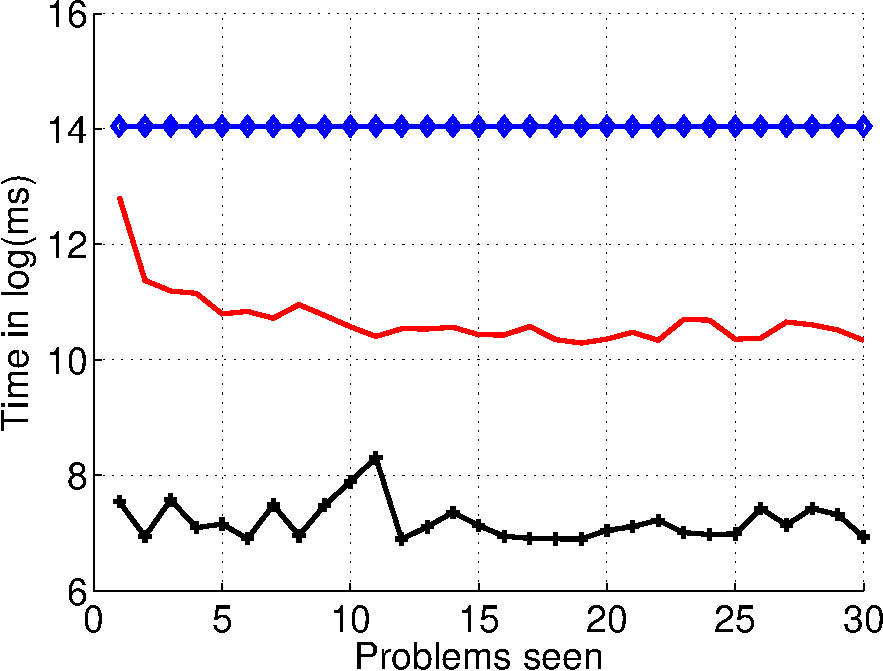
\includegraphics[width=14cm]{online/logistic_inference_time-crop}
  }
  \label{fig:logistic_performance}
\end{figure}

\textbf{Sampling + KJIT} = KJIT with an importance sampling oracle.

\end{block}

%--------------------------
\begin{block}{ Experiment 3: Compound Gamma Factor }
%--------------------------
Infer posterior of the precision $\tau$ of $x \sim \mathcal{N}(x; 0, \tau)$ 
from observations $\{x_i\}_{i=1}^N $:
%
\noindent
\begin{columns}[T]
   \hspace{-5cm}
   \begin{column}{1cm}
       \begin{align*}
          \textcolor{magenta}{r_2} &\sim \mathrm{Gamma}(r_2; s_1, r_1)  \\
          \tau &\sim \mathrm{Gamma}(\tau; s_2, \textcolor{magenta}{r_2} ) \\
          (s_1, r_1, s_2) &= (1, 1, 1).
       \end{align*}
   \end{column}
   %
   \hspace{-10cm}
   \begin{column}{1cm}
   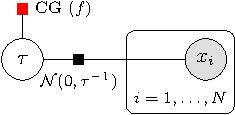
\includegraphics[width=11cm]{img/compound_gamma_graph-crop}
   \end{column}
\end{columns}

% compound gamma inferred results and time.
\begin{figure}[ht]
  \centering
% 	\subfloat[Posteriors]{
% 	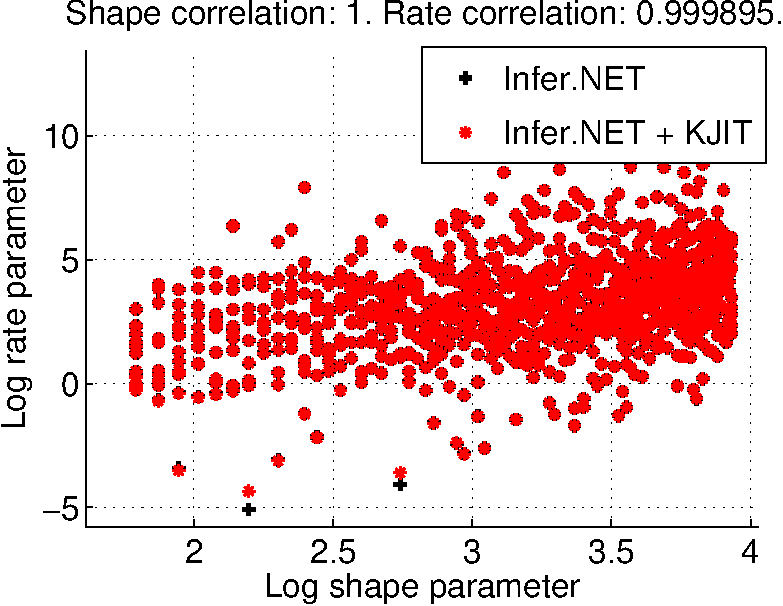
\includegraphics[width=0.49\columnwidth]{img/online/cg_post_corr-crop}
% 	%\missingfigure[figwidth=0.49\columnwidth]{}
% 	}
  %
  \subfloat[Inferred shape \label{fig:cg_infer_shape}]{
  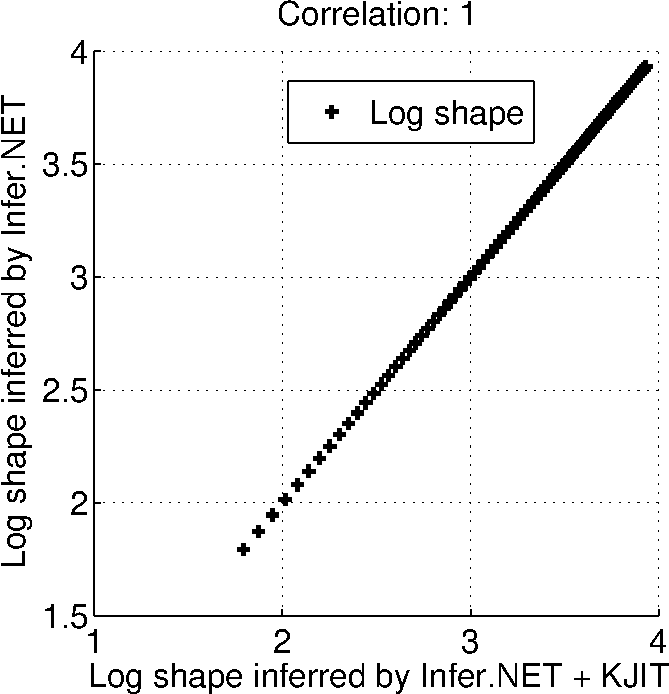
\includegraphics[width=11cm]{online/cg_post_shape-crop}
  %\missingfigure[figwidth=0.49\columnwidth]{}
  }
  %
  \subfloat[Inferred rate \label{fig:cg_infer_rate}]{
  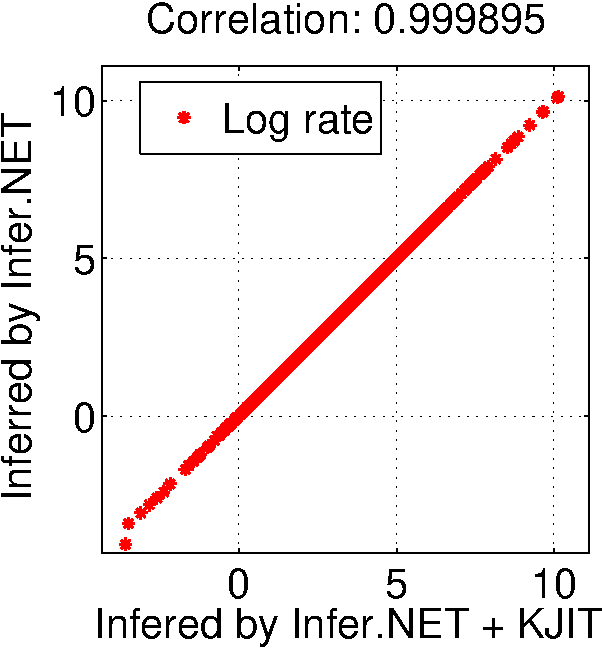
\includegraphics[width=11cm]{online/cg_post_rate-crop}
  %\missingfigure[figwidth=0.49\columnwidth]{}
  }
  %
  \subfloat[Inference time\label{fig:cg_infer_time}]{
  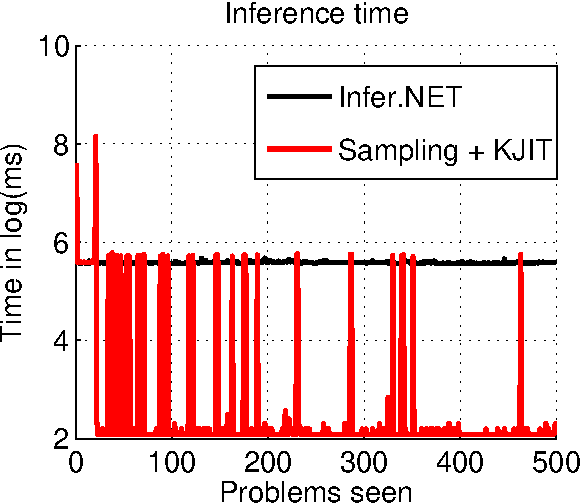
\includegraphics[width=11cm]{online/cg_inference_time-crop}
  }
  %\caption{Shape (a) and rate (b) parameters of the inferred posteriors in 
  %the compound gamma problem. 
  %(c) KJIT is able to infer equally good posterior parameters compared to Infer.NET 
  %while requiring a runtime several orders of magnitude lower. }
  \label{fig:cg_performance}
\end{figure}

\vspace{5mm}

\textbf{Inference quality}: as good as hand-crafted factor, much faster.
\end{block}

%--------------------------
\begin{block}{ Experiment 4: Real Data}
%--------------------------
\begin{itemize}
    \item Binary logistic regression.  Sequentially present 4 real datasets
        to the operator.
    \item Diverse distributions of incoming messages.
\end{itemize}

% UCI data classification error
% Inference time
\begin{figure}[ht]
  \centering
  \subfloat[Incoming messages]{
      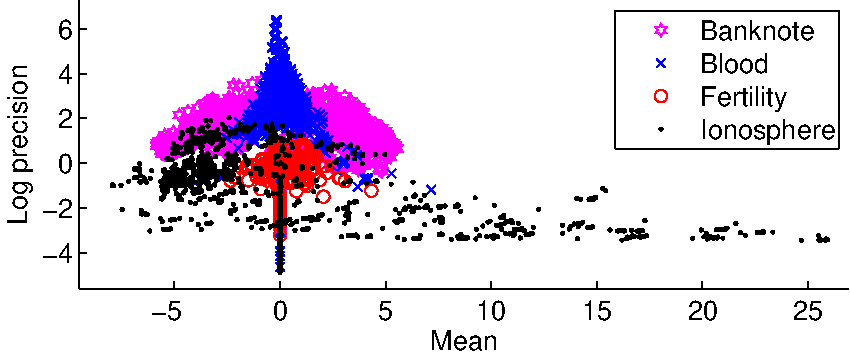
\includegraphics[width=0.32\columnwidth]{online/uci_in_msgs-crop}
  }
  %
  \subfloat[Test error\label{fig:uci_01_loss}]{
  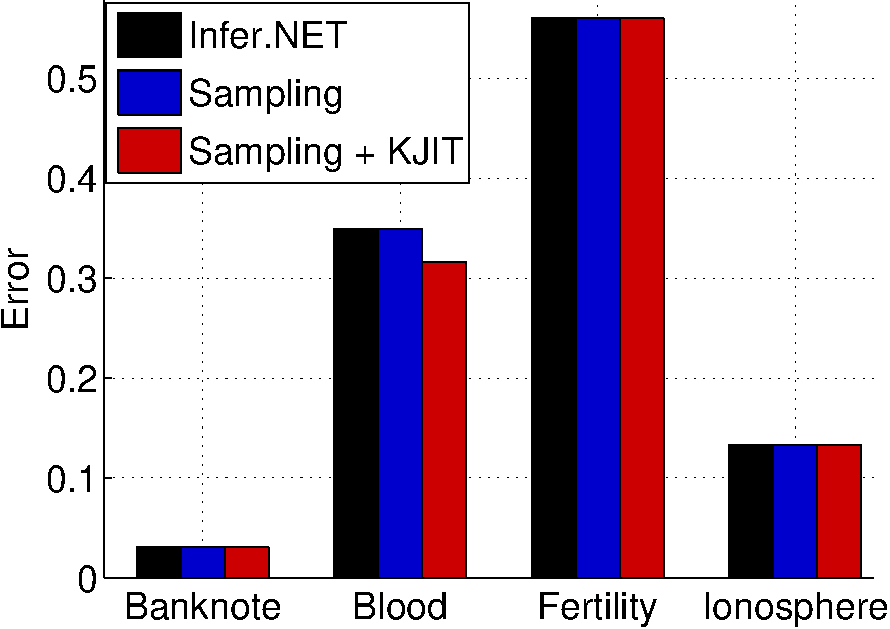
\includegraphics[width=0.31\columnwidth]{online/uci_classification-crop}
  }
  %
  \subfloat[Inference time\label{fig:uci_infer_time}]{
  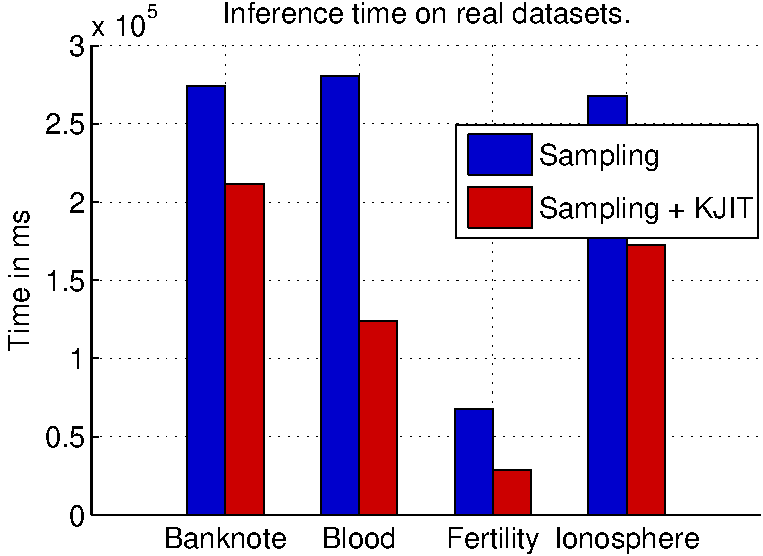
\includegraphics[width=0.31\columnwidth]{online/uci_infer_time-crop}
  }
  %\caption{Classification performance and inference times on the four UCI datasets.  }
  \label{fig:uci_performance}
\end{figure}

\begin{itemize}
    \item KJIT factor can adapt to the change of input message distributions.
\end{itemize}

% UCI datasets. temporal uncertainty.
\begin{figure}
\centering
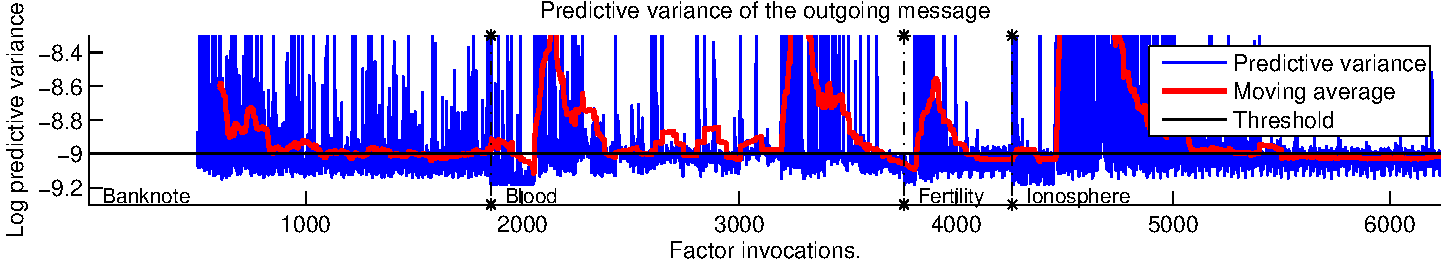
\includegraphics[width=0.99\textwidth]{online/uci_temporal_uncertainty-crop}
%\caption{
%Uncertainty estimate of KJIT for outgoing messages on the four UCI datasets.
%\label{fig:uci_temporal_uncertainty}
%}
\end{figure}

\end{block}



%%--------------------------
%\begin{block}{References}
%%--------------------------

%{\footnotesize
%\begin{enumerate}
%\item \justifying{} { A. Rahimi and B. Recht. Random Features
%for Large-scale Kernel Machines. NIPS 2007.}
%\item A. Smola et al. A Hilbert Space Embedding for Distributions. ALT 2007.
%\item { A. N. Heess et al. Learning to Pass Expectation Propagation Messages.
%NIPS 2013. }
%%\item T. Minka et al. Infer.NET. \url{http://research.microsoft.com/infernet}. 2012
%\item S. M. A. Eslami et al. Just-In-Time Learning for Fast and Flexible Inference.
%    NIPS 2014.
%\item A. Christmann and I. Steinwart. Universal kernels on non-standard input
%    spaces. NIPS 2010.
%\end{enumerate}
%}

%% \bibliographystyle{unsrt}
%% \bibliography{/nfs/nhome/live/wittawat/Dropbox/gatsby/paper_submission/kernel_ep_workshop/ref}


%\end{block}



\end{columns}

\end{frame}

\end{document}

